\section{Implementation of LTC n-dimension}
To implement LTC in nD with the infinity norm, we maintain a cuboid
representation of $\cap_{l=1}^j{\mathcal{B}_l}$ across the
iterations of the \texttt{while} loop in
Algorithm~\ref{algo:general-ltc}. The implementation works with
constant memory and requires limited CPU time.

With the Euclidean norm, the intersection test is more complex. We keep in
memory a growing set $S$ of balls and the bounding box $B$ of their
intersection. Then, when a new point arrives, we consider the associated ball
$\mathcal{B}_j$ and our intersection test works as in
Algorithm~\ref{algo:euclidean}. \texttt{box()} is a function that returns the
bounding box of an n-ball. \texttt{find\_bisection(S, B)} in
Algorithm~\ref{algo:find_bisection_function} and \texttt{recursive(S, L, R, N,
X)} in Algorithm~\ref{algo:recursive} searches for a point in all the  elements
in S, using plane sweep and bisection initialized by the bounds of B.


Different with Infinity norm, maintain balls intersection is not
straightforward. So in Euclidean norm, the function  \texttt{find\_bisection(S,
B)} will be invoked while receiving each new data  stream. The $B$ bounding box
in Euclidean norm is a cuboid but it just  represents a range the intersection
could be. With new associated ball  $\mathcal{B}_j$, we re-define it as follow:
\begin{equation*}
    B = \bigcap_{i=1}^{j-1} box(\mathcal{B}_i) 
\end{equation*}
Firstly, checking the intersection with box($\mathcal{B}_j$) and $B$, which
shows in Algorithm~\ref{algo:euclidean} line 9. Secondly, for each
$\mathcal{B}_i$ belongs to $S$, check the intersection between $\mathcal{B}_i$
and $\mathcal{B}_j$ (12 line in Algorithm~\ref{algo:euclidean}). At the same
time $\mathcal{B}_i$ will be removed if it includes $\mathcal{B}_j$, because
smaller ball intersects $\mathcal{B}_j$ than a bigger ball which contains the
smaller one(15 line in Algorithm~\ref{algo:euclidean}). Finally, finding a point
in intersection of balls in $S$ by running funtion \texttt{find\_bisection(S,
B)}.Our code is available at
\url{https://github.com/big-data-lab-team/stream-summarization} under MIT
license.



% describe function find_bisection
In function \texttt{find\_bisection(S, B)}, we selected dimension of balls as
$n$ used at the beginning of bisection, also computed minimum/maximum value of
bounding box $B$ at $n$ dimension, which corresponds to $left$ and $right$ in
bisection method. The $X$ represents a point in all elements in $S$. It would be
returned if it could be found in function \texttt{recursive(S, L, R, N, X)}.

% describe function recursive
The parameter $X$ put into function \texttt{recursive(S, L, R, N, X)}, because
it is necessary to update the values (see Algorithm~\ref{algo:recursive} line
28) of $X$ during the process. In 30 line of Algorithm~\ref{algo:recursive}, it
happens in case of $left > right$, which means:
\begin{equation*}
    mid \  \bigcap \  (min\_id \cap max\_id) = \O
\end{equation*}

In Algorithm~\ref{algo:euclidean} line 12, It denotes any two balls in $S$ has
intersection. Therefore, any point in the intersection of $min\_id$ and
$max\_id$, could be used for determining the direction of bisection. In our
implement, we select a point in connection of these two ball's center, which
also locates in intersecting object(line/chord when order=2, plane/circle when
order=3).Figure~\ref{fig:compare_point} shows the point we selected in 2D.


\note{Algorithm~\ref{algo:euclidean} line 9, code is box($B_j$), but not problem}
\note{line 16, remove $B_i$ from $S$, Add $B_j$ done in line 19}

\begin{algorithm}
\begin{algorithmic}[1]
\Input
    \Desc{$S$}{Set of intersecting balls}
    \Desc{$B$}{Bounding box of the intersection of balls in $S$}
    \Desc{$\mathcal{B}_j$}{New ball to check}
\EndInput
\Output
    \Desc{$S$}{Updated set of intersecting balls}
    \Desc{$B$}{Updated bounding box}
    \Desc{$T$}{True if all the balls in S and $\mathcal{B}_j$ intersect}
\EndOutput

%\If{$\mathcal{B}_j \cap B = \O$} \Comment{Ball is outside bounding box}
\If{box($\mathcal{B}_j$) $\cap B = \O$} \Comment{Ball is outside bounding box}
    \State \Return ($S$, $B$, False)
\EndIf
\If{$\exists\ \mathcal{B}_i \in S$ s.t. $\mathcal{B}_j \cap \mathcal{B}_i = \O$}
    \State \Return ($S$, False) \Comment{Some balls don't intersect}
\EndIf
\If{$\exists\ \mathcal{B}_i \in S$ s.t. $\mathcal{B}_j \subset \mathcal{B}_i$} \Comment{Remove inclusions}
%\State Remove $\mathcal{B}_i$ from $B$. %Add $\mathcal{B}_j$ to $B$. 
    \State Remove $\mathcal{B}_i$ from $S$. %Add $\mathcal{B}_j$ to $S$. 
\EndIf
\State $B$ = box($\mathcal{B}_j$) $\ \bigcap\ $ $B$
\State $S$ = $S \ \bigcup \  \{\mathcal{B}_j\}$
\State $x$ = find\_bisection($S$, $B$) \Comment{This can take some time}
\If{$x$ == Null}
    \State \Return ($S$, $B$, False)
\Else
    \State \Return ($S$, $B$, True)
\EndIf
\end{algorithmic}
\caption{Intersection test for Euclidean n-balls.}
\label{algo:euclidean}
\end{algorithm}


\begin{comment}
In Euclidean distance version, we also map the coming data into same
time-stamp $t_1$ the timestamp after base point. The difference with
Manhattan distance version is that recording overlapping part with
a post-designed model is difficult, which need retain several arcs in
2-dimension, or convex surfaces in 3-dimension. In our method, we will
record all tolerance range for every mapped data which come from base
data point until coming data point, in order to checking if there is
intersection among them. For instance, in 3D-t, assume we have a the	
base point $Z = D_0$ and the tolerance range $R_1$ which is a ball
as the intersection S. we need a list L to record mapped balls
from $D_1$ to coming data. For each comming data $D_i, i>1$ mapping
this data into $t_1$, and add it into list. Then the work is check out
if all balls intersect, and form a public intersection. The method is
based on plane sweep and binary search. At first, select one parameter,
such as x-axis, finding a bounding range of all balls $B_i$ in x-axis.
suppose $Max_bound_x = Min{1..n}{B_i.center.x + EPSILON/i}$, and
$Min_bound_x = Max{1..n}{B_i.center.x - EPSILON/i}$. If there is overlap
among balls, then the axis of the points inside intersection must located
between Min_bound_x and Max_bound_x. Using binary search to select
mid_x = (Min_bound_x + Max_bound_x)/2, then calculate a y-axis bounding
with the plane x = mid_x. If the get bounding range in y-axis where
$Max_bound_y > Min_bound_y$ and using binary search again to find mid_y,
It means there is a line x=mid_x, Max_bound_y>= y >= Min_bound_y,
parallels z-axis, could pass through all balls. Finally, in z-axis,
computing bounding range, and If $Max_bound_z > Min_bound_z$, there
must be one or more points inside all balls. The problem be solved.
If the loop of binary search in x-axis overs, then there is no public
intersection among balls, and need to transmit and update base point.
In this method we need O(n*logn*logn) time complexity for binary search
in x-axis and y-axis and traversal all balls in z-axis, also O(n) space
complexity is needed for maintaining list. According this method,
it could be extended into N-dimensional data. The main idea is to search,
dimension by dimension, from a room or plane or line and get intersection
point finally.
\end{comment}


\begin{algorithm}
\begin{algorithmic}[1]
\Input
   \Desc{$S$}{Set of intersecting balls}
   \Desc{$B$}{Bounding box of the intersection of balls in $S$}
\EndInput
\Output
   \Desc{$X$}{Point in all balls in $S$, $X = \{x_1,...,x_n\}$}
\EndOutput

\State $n$ = dimension of balls
\State $left$ = min\_value($B$, $n$) \Comment{Minimum value of $B$ at $n_{th}$ dimension}
\State $right$ = max\_value($B$, $n$) \Comment{Maximum value of $B$ at $n_{th}$ dimension}
\If{recursive(S, left, right, n, X)}
    \State \Return $X$
\Else
    \State \Return Null
\EndIf
\end{algorithmic}
\caption{Function find\_bisection(S, B)}
\label{algo:find_bisection_function}
\end{algorithm}


%\todo{check this algorithm}
\begin{algorithm}
\begin{algorithmic}[1]
\Input
   \Desc{$S$}{Set of intersecting balls}
   \Desc{$L$}{Min value used in bisection}
   \Desc{$R$}{Max value used in bisection}
   \Desc{$N$}{The $N_{th}$ dimension, $N \in \{1...n\}$}
   \Desc{$X$}{Point in all balls in $S$, $X = \{x_1,...,x_n\}$}
\EndInput
\Output
   \Desc{$T$}{True if a point be found by using bisection}
\EndOutput
\If{$N$ == 1}
    \State $X.x_1$ = $\frac{L+R}{2}$
    \State \Return True
\EndIf
\While{$L \leqslant R$ }
    \State $mid$ = $\frac{L+R}{2}$
    \State $surface$ = $\{x_{N}...x_{n}\}$
    \State $left$ = -$\infty$, $\ right$ = +$\infty$
    \ForAll{$\mathcal{B}_i \in S$}
        \State $min$ = min\_value($\mathcal{B}_i \cap surface$, N-1)
        \State $max$ = max\_value($\mathcal{B}_i \cap surface$, N-1)
        \If{$left < min$}
            \State $left$ = $min$, $\ min\_id$ = $\mathcal{B}_i$
        \EndIf
        \If{$right > max$}
            \State $right$ = $max$, $\ max\_id$ = $\mathcal{B}_i$
        \EndIf
    \EndFor
    
    \If{$left \leqslant right$}
        \State $X.x_N$ = $mid$
        \State \Return recursive($S$, $left$, $right$, $N-1$, $X$)
    \ElsIf{$\ \forall\ P$ (Point) $\in (min\_id \cap max\_id)$ s.t. $P.x_N < mid$}
        \State $right$ = $mid$
    \Else
        \State $left$ = $mid$
    \EndIf
\EndWhile
\State \Return False
\end{algorithmic}
\caption{Function recursive(S, L, R, N, X)}
\label{algo:recursive}
\end{algorithm}

\section{Implementation of Polynomial Regression}

We implement polynomial regression method to compress the accelerometer data
($a.x$, $a.y$, $a.z$). In the dataset, we process polynomial regression with the
relationship between independent variable $t$ and dependent variables $a.x$,
$a.y$ and $a.z$. For tolerance checking, we use infinity norm and euclidean
norm. The implementation works need small memory to record data points, and some
CPU time to compute coefficients.

\begin{figure}
  \centering
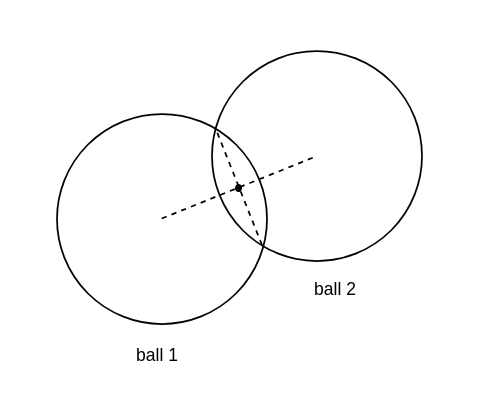
\includegraphics[width=0.7\textwidth]{figures/point-in-chord.png}
\caption{The point selected to determine the direction}
\label{fig:compare_point}
\end{figure}
